% Options for packages loaded elsewhere
\PassOptionsToPackage{unicode}{hyperref}
\PassOptionsToPackage{hyphens}{url}
%
\documentclass[
]{article}
\usepackage{lmodern}
\usepackage{amssymb,amsmath}
\usepackage{ifxetex,ifluatex}
\ifnum 0\ifxetex 1\fi\ifluatex 1\fi=0 % if pdftex
  \usepackage[T1]{fontenc}
  \usepackage[utf8]{inputenc}
  \usepackage{textcomp} % provide euro and other symbols
\else % if luatex or xetex
  \usepackage{unicode-math}
  \defaultfontfeatures{Scale=MatchLowercase}
  \defaultfontfeatures[\rmfamily]{Ligatures=TeX,Scale=1}
\fi
% Use upquote if available, for straight quotes in verbatim environments
\IfFileExists{upquote.sty}{\usepackage{upquote}}{}
\IfFileExists{microtype.sty}{% use microtype if available
  \usepackage[]{microtype}
  \UseMicrotypeSet[protrusion]{basicmath} % disable protrusion for tt fonts
}{}
\makeatletter
\@ifundefined{KOMAClassName}{% if non-KOMA class
  \IfFileExists{parskip.sty}{%
    \usepackage{parskip}
  }{% else
    \setlength{\parindent}{0pt}
    \setlength{\parskip}{6pt plus 2pt minus 1pt}}
}{% if KOMA class
  \KOMAoptions{parskip=half}}
\makeatother
\usepackage{xcolor}
\IfFileExists{xurl.sty}{\usepackage{xurl}}{} % add URL line breaks if available
\IfFileExists{bookmark.sty}{\usepackage{bookmark}}{\usepackage{hyperref}}
\hypersetup{
  hidelinks,
  pdfcreator={LaTeX via pandoc}}
\urlstyle{same} % disable monospaced font for URLs
\usepackage[margin=1in]{geometry}
\usepackage{graphicx}
\makeatletter
\def\maxwidth{\ifdim\Gin@nat@width>\linewidth\linewidth\else\Gin@nat@width\fi}
\def\maxheight{\ifdim\Gin@nat@height>\textheight\textheight\else\Gin@nat@height\fi}
\makeatother
% Scale images if necessary, so that they will not overflow the page
% margins by default, and it is still possible to overwrite the defaults
% using explicit options in \includegraphics[width, height, ...]{}
\setkeys{Gin}{width=\maxwidth,height=\maxheight,keepaspectratio}
% Set default figure placement to htbp
\makeatletter
\def\fps@figure{htbp}
\makeatother
\setlength{\emergencystretch}{3em} % prevent overfull lines
\providecommand{\tightlist}{%
  \setlength{\itemsep}{0pt}\setlength{\parskip}{0pt}}
\setcounter{secnumdepth}{-\maxdimen} % remove section numbering
\usepackage{ctex}
\usepackage{xcolor}
\usepackage{fancyhdr}
\pagestyle{plain}
\usepackage{sectsty}
\definecolor{glaucous}{rgb}{0.38, 0.51, 0.71}
\definecolor{lavenderblush}{rgb}{1.0, 0.94, 0.96}
\definecolor{grey}{RGB}{96, 96, 96}
\usepackage{enumitem}% http://ctan.org/pkg/enumitem
\usepackage[empty]{fullpage}% http://ctan.org/pkg/fullpage
\usepackage{color}% http://ctan.org/pkg/color
\usepackage{hyperref}% http://ctan.org/pkg/hyperref
\usepackage{geometry}
\geometry{papersize={15.5cm,400cm},left=0.5cm,right=0.5cm,top=0.3cm,bottom=0.3cm}
\usepackage{blindtext}
\usepackage[center]{caption}
\usepackage[font=Large]{caption}
\usepackage{subfigure}
\usepackage{float}
\usepackage{graphicx}
\usepackage{booktabs}
\usepackage[justification=centering]{caption}
\usepackage{threeparttable}
\usepackage{longtable}
\usepackage{array}
\usepackage{multirow}
\usepackage{wrapfig}
\usepackage{float}
\usepackage{colortbl}
\usepackage{pdflscape}
\usepackage{tabu}
\usepackage{threeparttable}
\usepackage{threeparttablex}
\usepackage[normalem]{ulem}
\usepackage{makecell}
\usepackage{xcolor}
\linespread{1.85}
\setlength{\parskip}{1em}
\setlength{\footskip}{20pt}
\setCJKmainfont[BoldFont=SimHei,ItalicFont=KaiTi]{微软雅黑}
\usepackage{booktabs}
\usepackage{longtable}
\usepackage{array}
\usepackage{multirow}
\usepackage{wrapfig}
\usepackage{float}
\usepackage{colortbl}
\usepackage{pdflscape}
\usepackage{tabu}
\usepackage{threeparttable}
\usepackage{threeparttablex}
\usepackage[normalem]{ulem}
\usepackage{makecell}
\usepackage{xcolor}

\author{}
\date{\vspace{-2.5em}}

\begin{document}

\captionsetup[figure]{name={图},labelsep=space}
\captionsetup[table]{name={表},labelsep=space} 
\fontsize{22}{22}
\selectfont
\vspace{-10truemm}

\newcommand{\resheading}[1]{%
  \noindent\fcolorbox{lavenderblush}{lavenderblush}{\makebox[\dimexpr\textwidth-2\fboxsep-2\fboxrule][c]{\textbf{~#1}}}%
}

\begin{center}

\includegraphics[height=2cm]{./input/logo2.png} 
\end{center}

\begin{center}
\fontsize{45}{45}
\textcolor{glaucous}{\textbf{新冠早报}}
\end{center}

\begin{center}
\fontsize{22}{22}
{\textcolor{glaucous}{\textbf{第72期 \space 6月30日}}}
\end{center}

\begin{center}

\includegraphics[height=2cm]{./input/title1.png} 
\end{center}

\vspace{-5mm}

\hypertarget{section}{%
\subsection{\texorpdfstring{\textcolor{glaucous}{\Huge 国际}}{}}\label{section}}

\vspace{-3mm}

\begin{center}
\textcolor{glaucous}{英国广播公司(BBC)}\\纽约州长制定五月重新开放的计划

\end{center}

据当地时间4月28日报道,美国纽约州州长安德鲁·库莫称,纽约州部分地区若满足解禁条件(包括连续14天新冠病例下降),则5月15日可以开始放宽新冠限制措施。但医院容纳量在70%以上,或新冠传染率高于1.1的地区都不能重新开放。如果制造业和建筑业能够采取充分预防措施,它们将会是首批重新开放的企业。

\begin{center}
\textcolor{glaucous}{美国有线电视新闻网(CNN)}\\特朗普命令肉类加工厂保持开放
\end{center}

当地时间4月28日,美国总统特朗普称,他将根据《国防生产法》签署一项五页的行政命令,保持肉类加工厂在冠状病毒大流行中继续开放。此命令是在一些公司(例如泰森食品公司)考虑只开放其20%的设施之后签署的。美国政府还将与劳工部合作,发布对有关对肉类加工厂雇员的居家指导。

\begin{center}
\textcolor{glaucous}{英国广播公司(BBC)}\\英国将扩大面向护理机构员工和65岁以上老人的新冠测试
\end{center}

当地时间4月28日,英国卫生部长马特·汉考克称,英国所有疗养院居民和工作人员,不论是否有症状,都将符合新冠检测的资格。从4月29日开始,所有有症状的65岁以上以及必须出门上班的人,也可以接受检查。汉考克称,现在英国每日测试能力高达73,400,到五月,政府每天将进行10万次测试。

\begin{center}
\textcolor{glaucous}{纽约时报(New York Times)}\\西班牙,法国和希腊公布放宽新冠限制措施计划

\end{center}

据美东时间4月28日报道,西班牙总理佩德罗·桑切斯宣布,自5月2日起,成年人可以在户外运动。限制措施的放宽将因地区而异,但学校不会在9月之前重新开放。希腊总理基里亚科斯·米佐塔基斯表示,5月4日开始,希腊人可以自由离开家,届时一些商店将重新营业,但沙龙将仅通过预约开放,教堂将开放但不能举行礼拜,人们可以去海滩运动,高中生将从5月11日起分阶段重返学校。法国总理爱德华·菲利普称,如果新冠疫情持续得到控制,政府将在5月11日开始放宽限制措施,并于6月2日重新评估这些措施。

\begin{center}
\textcolor{glaucous}{英国广播公司(BBC)}\\特朗普承诺向尼日利亚提供呼吸机

\end{center}

当地时间4月28日,尼日利亚政府官员在每日新闻发布会上表示,既美国总统特朗普承诺向厄瓜多尔提供呼吸机后,其首次承诺向尼日利亚等西非国家提供呼吸机,帮助其应对冠状病毒的流行。

\begin{center}
\textcolor{glaucous}{NA}NA
\end{center}

NA

\vspace{5mm}

\hypertarget{section-1}{%
\subsection{\texorpdfstring{\textcolor{glaucous}{\Huge 国内}}{}}\label{section-1}}

\vspace{-3mm}

\begin{center}
\textcolor{glaucous}{中国新闻网}\\小汤山医院新冠肺炎患者全部“清零”

\end{center}

北京时间4月28日上午,随着最后两名患者顺利出院,小汤山医院新冠肺炎患者全部``清零'',首批912名医务人员零感染回家。

\begin{center}
\textcolor{glaucous}{美国公共广播电台(NPR)}\\北京批评印度取消中国抗体检测试剂盒订单是“不公正”的决定
\end{center}

当地时间4月27日,印度医药研究议会建议停止使用从中国广州万孚生物技术和珠海丽珠试剂公司生产的抗体检测试剂盒,并将65万个抗体检测试剂盒的订单退回中国供应商。该议会声称这批抗体检测试剂盒的检测敏感性差异较大。北京时间4月28日,中国驻新德里使馆发言人吉荣批评印度取消进口中国抗体检测试剂盒订单的决定,坚持测试剂盒已经过验证和批准。他在声明中称:``某些人将中国产品标记为`有缺陷',并以固有偏见看待这些问题是不公平和不负责任的。''

\vspace{5mm}

\begin{center}

\includegraphics[height=2cm]{./input/title2.png} 
\end{center}

\begin{Large}
\vspace{-7mm}
{数据源:约翰霍普金斯大学,The COVID Tracking  Project}
\end{Large}

\vspace{-7mm}

\begin{Large}
{数据截止至:北京时间6月30日 上午8:00}
\end{Large}

\vspace{-7mm}

\hypertarget{section-2}{%
\section{\texorpdfstring{\textcolor{glaucous}{\Huge 一、世界疫情}}{}}\label{section-2}}

\vspace{-5mm}

\(\bullet\)全球累计确诊病例达到10,815,117例,累计死亡519,575例。共有31个国家累计确诊病例数超过5万例,其中10个为欧洲国家,10个为亚洲国家,9个为美洲国家,另有两个非洲国家。

\(\quad\)\(\diamond\)北美洲确诊病例数持续增长,已超过320万例,排名第一。

\(\quad\)\(\diamond\)南美洲地区疫情蔓延迅速,确诊病例数超过230万例,超过亚洲。

\begin{figure}[H]
\captionsetup{font={huge}}
\caption{\textcolor{grey}{世界疫情分布趋势图(来源:WHO)}} %最终文档中希望显示的图片标题
\centering
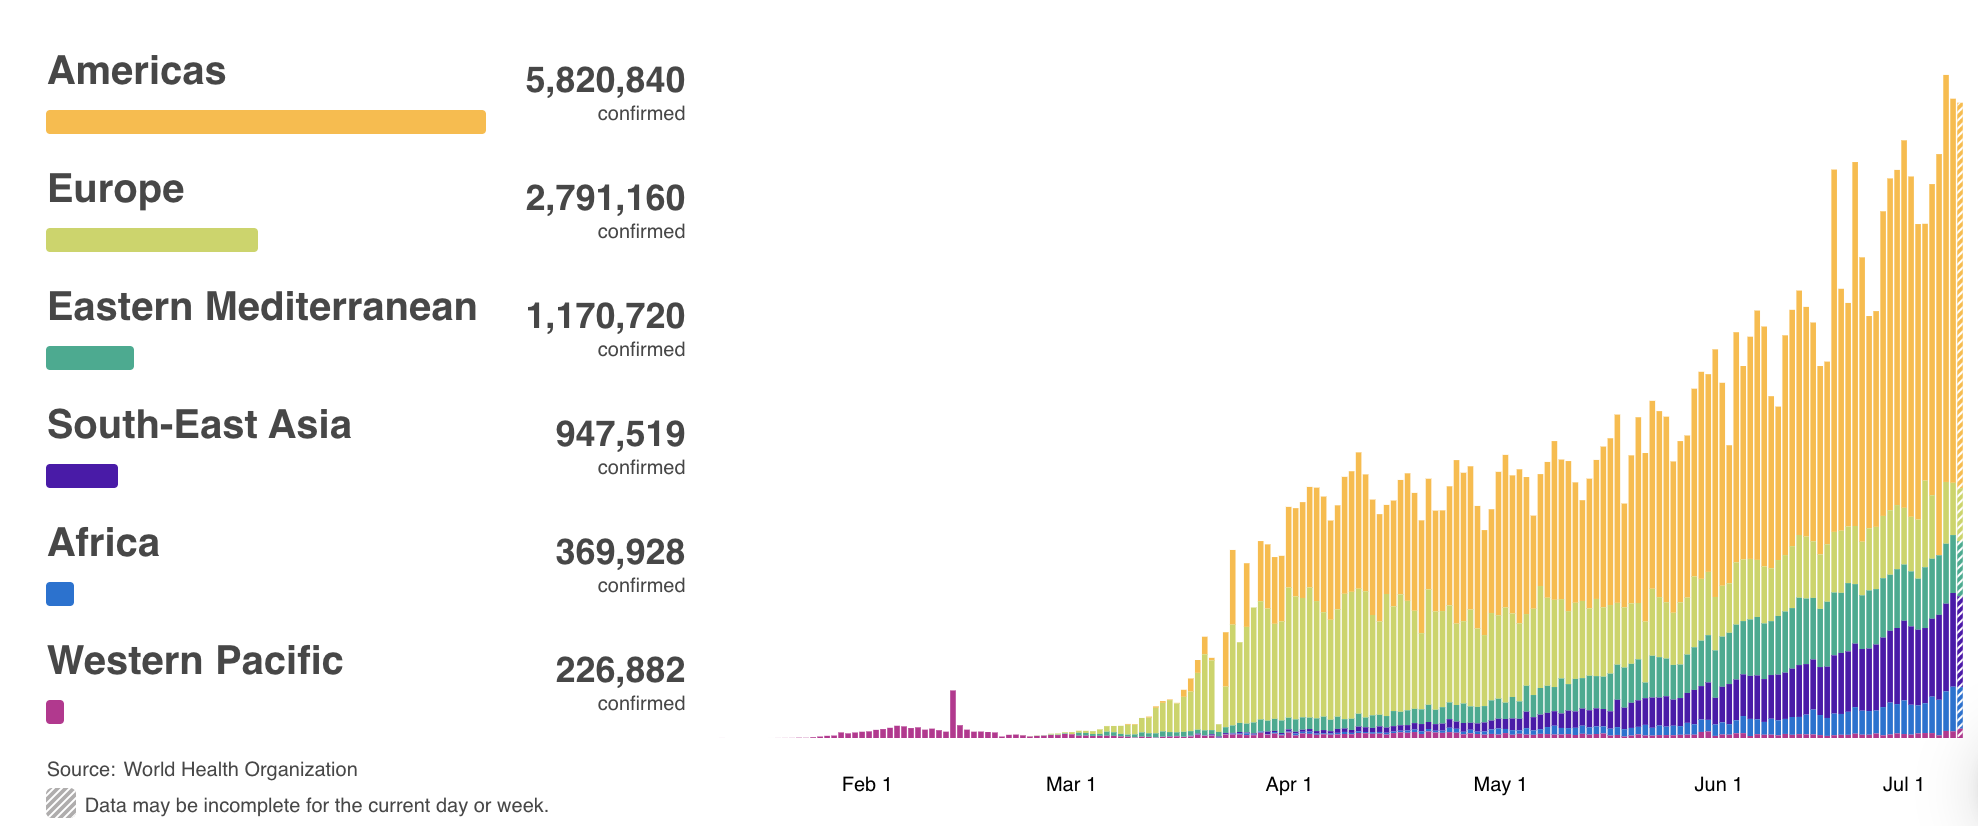
\includegraphics[]{./input/covid1.png} %插入图片,[]中设置图片大小,{}中是图片文件名
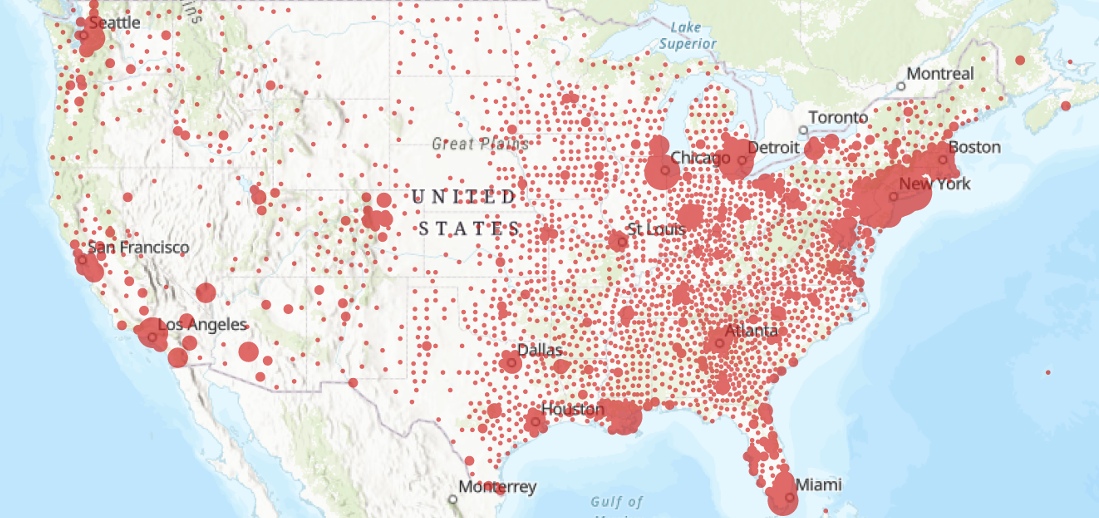
\includegraphics[]{./input/covid4.png}
\label{} %用于文内引用的标签
\end{figure}

\begin{table}[H]
    \centering \begin{table}[H]
\centering\begingroup\fontsize{20}{22}\selectfont

\begin{tabular}{rlrr}
\toprule
\multicolumn{0}{c}{\textbf{ }} & \multicolumn{3}{c}{\textbf{表1 累计确诊前十位国家}} \\
  & 国家(地区) & 累计确诊病例 & 粗发病率*\\
\midrule
\rowcolor{gray!6}  1 & 美国 US & 1,132,512 & 342\\
2 & 西班牙 Spain & 216,582 & 463\\
\rowcolor{gray!6}  3 & 意大利 Italy & 209,328 & 346\\
4 & 英国 UK & 183,500 & 270\\
\rowcolor{gray!6}  5 & 法国 France & 169,053 & 259\\
6 & 德国 Germany & 164,967 & 197\\
\rowcolor{gray!6}  7 & 土耳其 Turkey & 124,375 & 147\\
8 & 俄罗斯 Russia & 124,054 & 85\\
\rowcolor{gray!6}  9 & 巴西 Brazil & 96,559 & 45\\
10 & 伊朗 Iran & 96,448 & 115\\
\bottomrule
\end{tabular}
\endgroup{}
\end{table} \end{table}\begin{table}[H]
    \centering \begin{table}[H]
\centering\begingroup\fontsize{20}{22}\selectfont

\resizebox{\linewidth}{!}{
\begin{tabular}{rlrr}
\toprule
\multicolumn{0}{c}{\textbf{ }} & \multicolumn{3}{c}{\textbf{表2 粗发病率前十位国家}} \\
  & 国家(地区) & 粗发病率* & 累计确诊病例\\
\midrule
\rowcolor{gray!6}  1 & 圣马力诺 San Marino & 1,709 & 580\\
2 & 梵蒂冈 Holy See & 1,373 & 11\\
\rowcolor{gray!6}  3 & 安道尔 Andorra & 967 & 747\\
4 & 卢森堡 Luxembourg & 609 & 3,812\\
\rowcolor{gray!6}  5 & 冰岛 Iceland & 527 & 1,798\\
6 & 卡塔尔 Qatar & 516 & 14,872\\
\rowcolor{gray!6}  7 & 西班牙 Spain & 463 & 216,582\\
8 & 爱尔兰 Ireland & 429 & 21,176\\
\rowcolor{gray!6}  9 & 比利时 Belgium & 427 & 49,517\\
10 & 意大利 Italy & 346 & 209,328\\
\bottomrule
\end{tabular}}
\endgroup{}
\end{table} \begin{tablenotes}
        \fontsize{15}{15}
        \selectfont
        \item 注:*粗发病率定义:在一定时间内,特定范围人群中某病新发生的病例出现的频率。计算方式:(累计确诊病例/人口)×10万;国家人口不足 10 万人未列出 %此处加入注释信息
      \end{tablenotes}
\end{table}

\(\bullet\)全球昨日新增确诊接近19万例(18,8417例)(图2和表3),新增死亡4,033例(图3和表4)。

\(\quad\)\(\diamond\)北美洲新增确诊接近5万例,新增死亡病例616例。其中美国疫情依旧严重,新增确诊超过5.3万例(表3和表5为霍普金斯大学官网截至北京时间7月3日早8:00所更新的数据)。

\(\quad\)\(\diamond\)南美洲新增确诊超过5万例,新增死亡病例已超过1,500例,约70\%的新增确诊和约60\%新增死亡病例来自巴西,其余国家中秘鲁和哥伦比亚为主要疫情国家,当日新增确诊均超过3000例。

\(\quad\)\(\diamond\)亚洲新增确诊超过4万例,新增死亡482例,其中印度新增确诊接近2万例,约占50\%,另外巴基斯坦和孟加拉国新增确诊均超过4,000。

\(\quad\)\(\diamond\)非洲新增确诊超过1.3万例,新增死亡259例。南非疫情持续扩散,单日新增确诊病例接近9,000例。

\begin{table}[H]
    \centering \begin{table}[H]
\centering\begingroup\fontsize{20}{22}\selectfont

\begin{tabular}{rlr}
\toprule
\multicolumn{0}{c}{\textbf{ }} & \multicolumn{2}{c}{\textbf{表3 日新增病例前十位国家}} \\
  & 国家 & 当日新增病例\\
\midrule
\rowcolor{gray!6}  1 & 美国 US & 23,403\\
2 & 俄罗斯 Russia & 6,411\\
\rowcolor{gray!6}  3 & 巴西 Brazil & 4,440\\
4 & 英国 UK & 4,002\\
\rowcolor{gray!6}  5 & 法国 France & 3,089\\
6 & 西班牙 Spain & 2,706\\
\rowcolor{gray!6}  7 & 秘鲁 Peru & 2,491\\
8 & 土耳其 Turkey & 2,392\\
\rowcolor{gray!6}  9 & 意大利 Italy & 2,091\\
10 & 印度 India & 1,909\\
\bottomrule
\end{tabular}
\endgroup{}
\end{table} \end{table}\begin{table}[H]
    \centering \begin{table}[H]
\centering\begingroup\fontsize{20}{22}\selectfont

\resizebox{\linewidth}{!}{
\begin{tabular}{rlrrr}
\toprule
\multicolumn{0}{c}{\textbf{ }} & \multicolumn{4}{c}{\textbf{表4 累计死亡病例前十位国家}} \\
  & 国家 & 累计死亡病例 & 较昨日新增 & 病死率\%\\
\midrule
\rowcolor{gray!6}  1 & 美国 US & 58,343 & 2,084 & 5.8\\
2 & 意大利 Italy & 27,359 & 382 & 13.6\\
\rowcolor{gray!6}  3 & 西班牙 Spain & 23,822 & 301 & 10.3\\
4 & 法国 France & 23,694 & 367 & 14.0\\
\rowcolor{gray!6}  5 & 英国 UK & 21,745 & 588 & 13.4\\
6 & 比利时 Belgium & 7,331 & 124 & 15.5\\
\rowcolor{gray!6}  7 & 德国 Germany & 6,280 & 154 & 3.9\\
8 & 伊朗 Iran & 5,877 & 71 & 6.3\\
\rowcolor{gray!6}  9 & 巴西 Brazil & 5,017 & 414 & 7.0\\
10 & 中国 China & 4,637 & 0 & 5.5\\
\bottomrule
\end{tabular}}
\endgroup{}
\end{table} \begin{tablenotes}
        \fontsize{15}{15}
        \selectfont
        \item 
      \end{tablenotes}
\end{table}

\begin{figure}[H]
\centering
\captionsetup{font={huge}}
\caption{\textcolor{grey}{日新增确诊病例国家趋势图}}
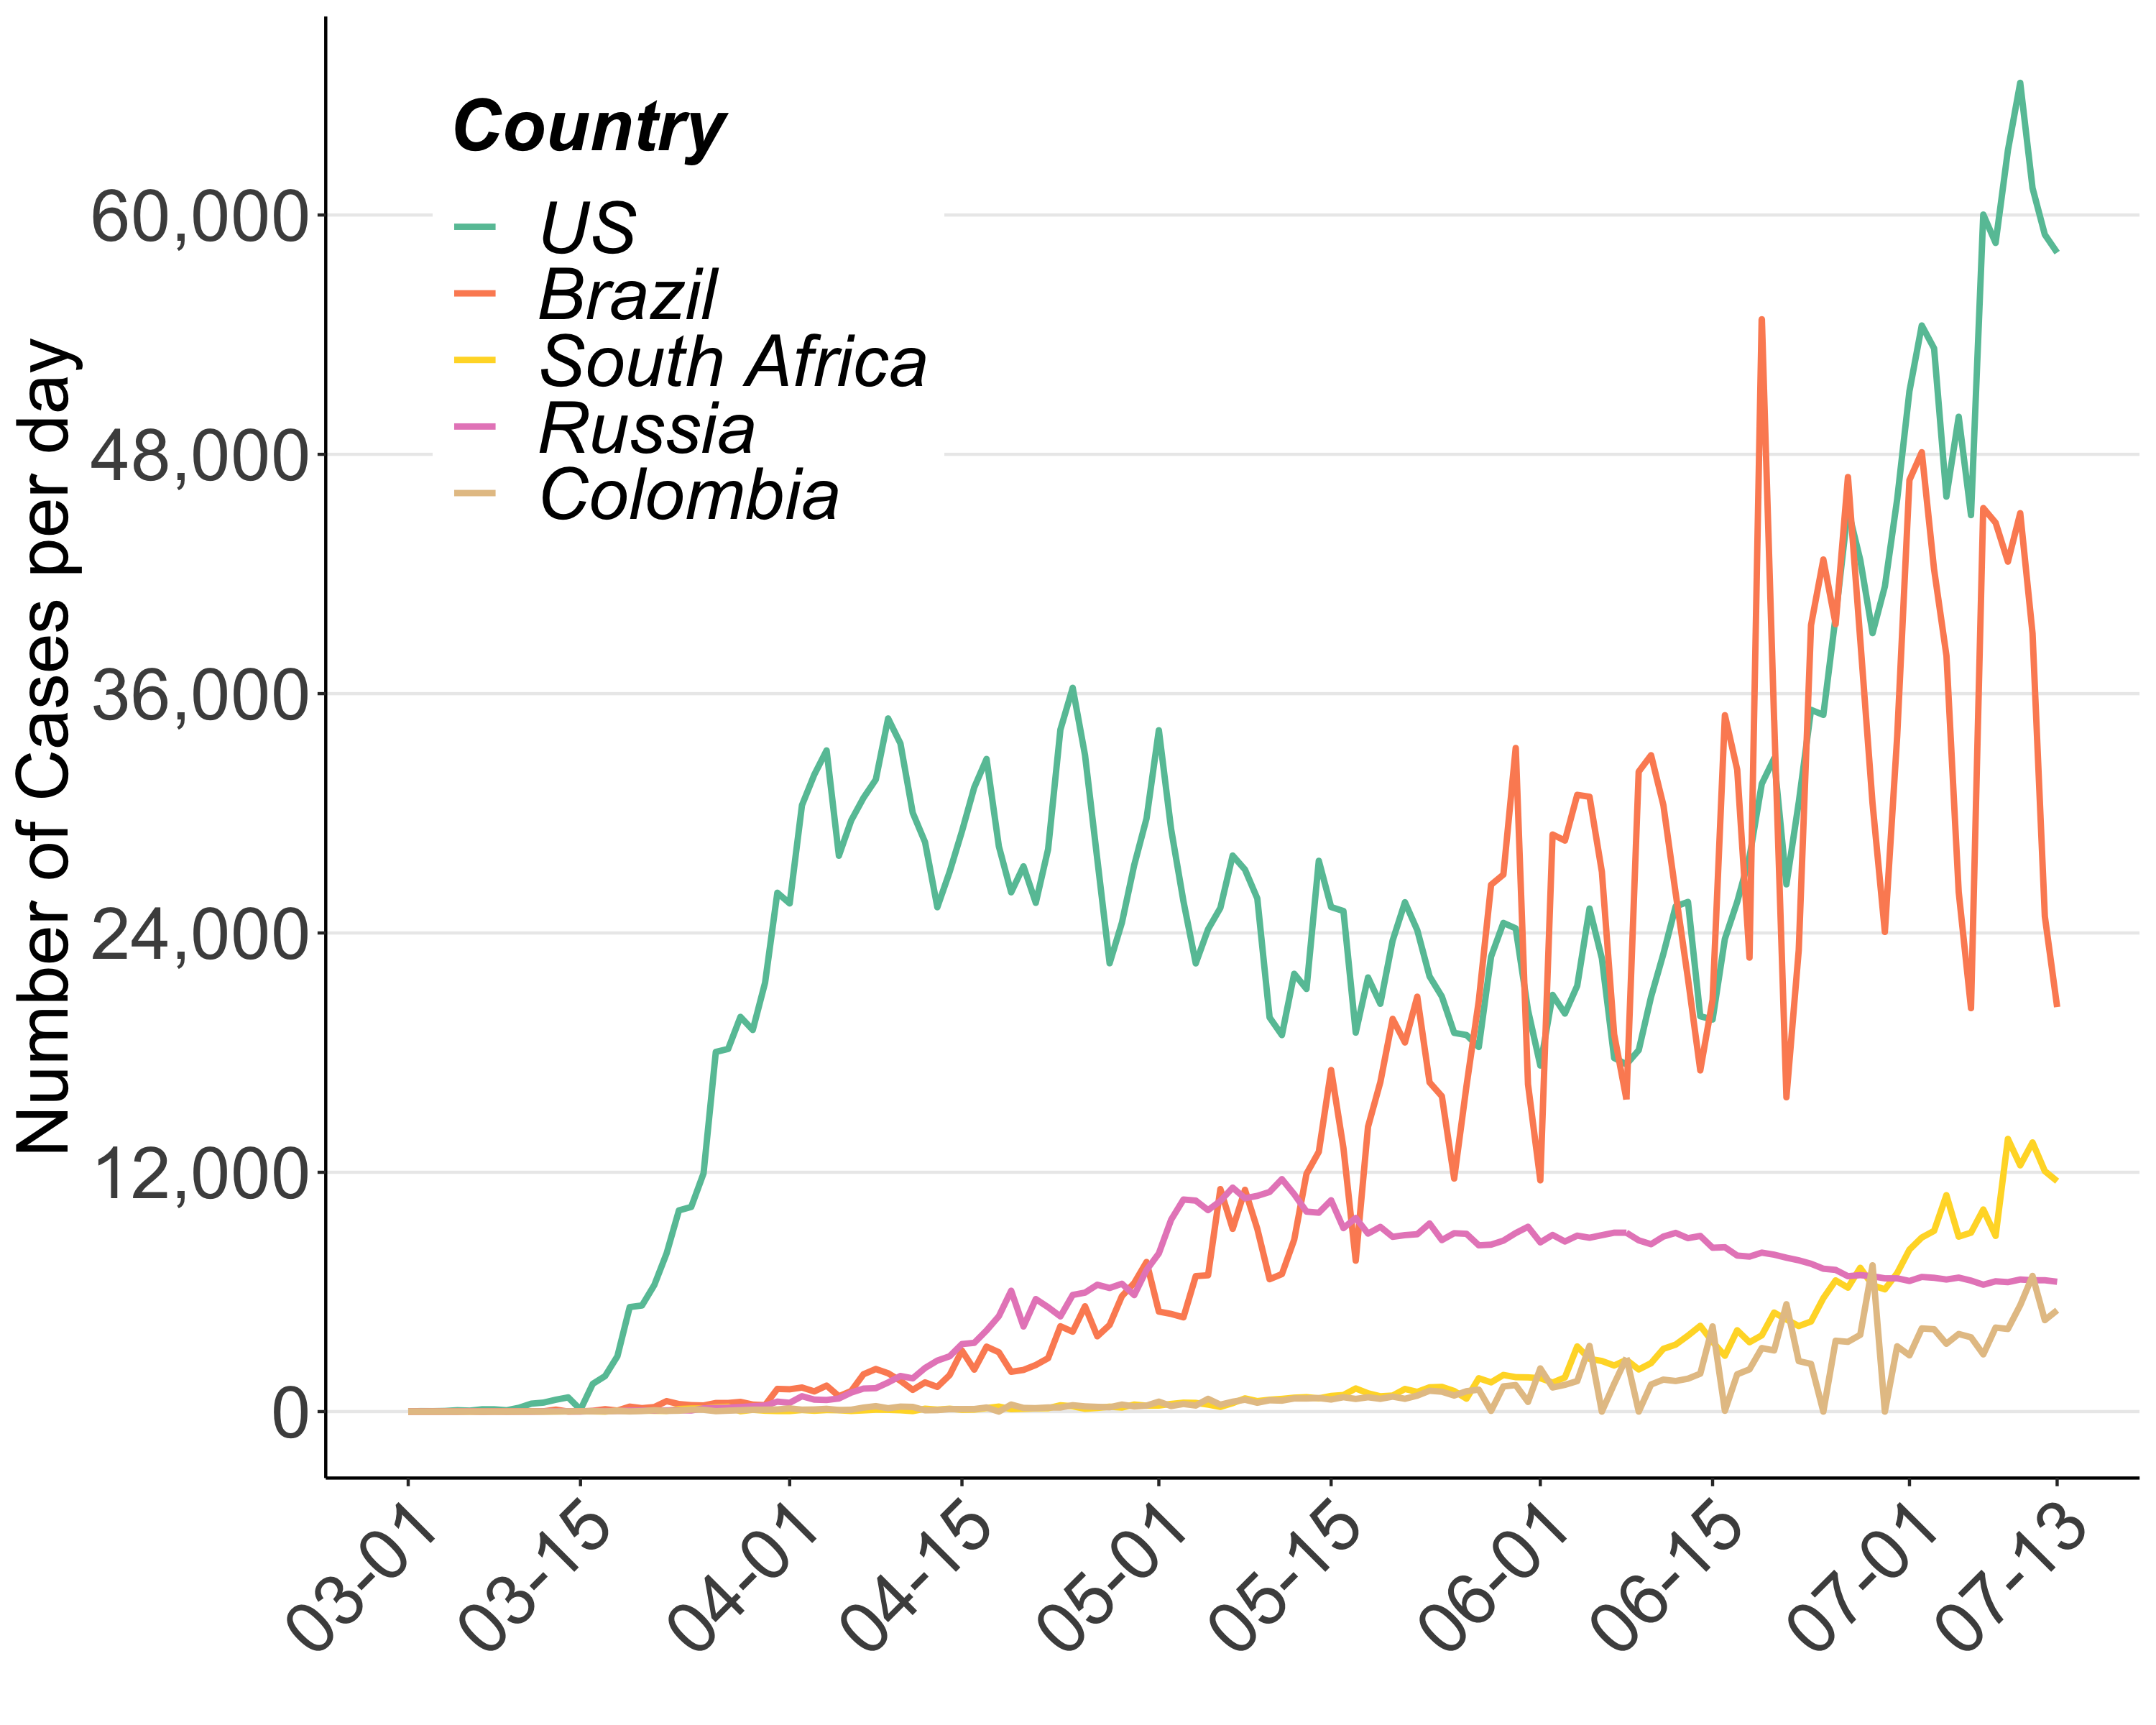
\includegraphics[]{./input/covid2.png}
\end{figure}

\begin{figure}[H]
\centering
\captionsetup{font={huge}}
\caption{\textcolor{grey}{日新增死亡病例国家趋势图}}
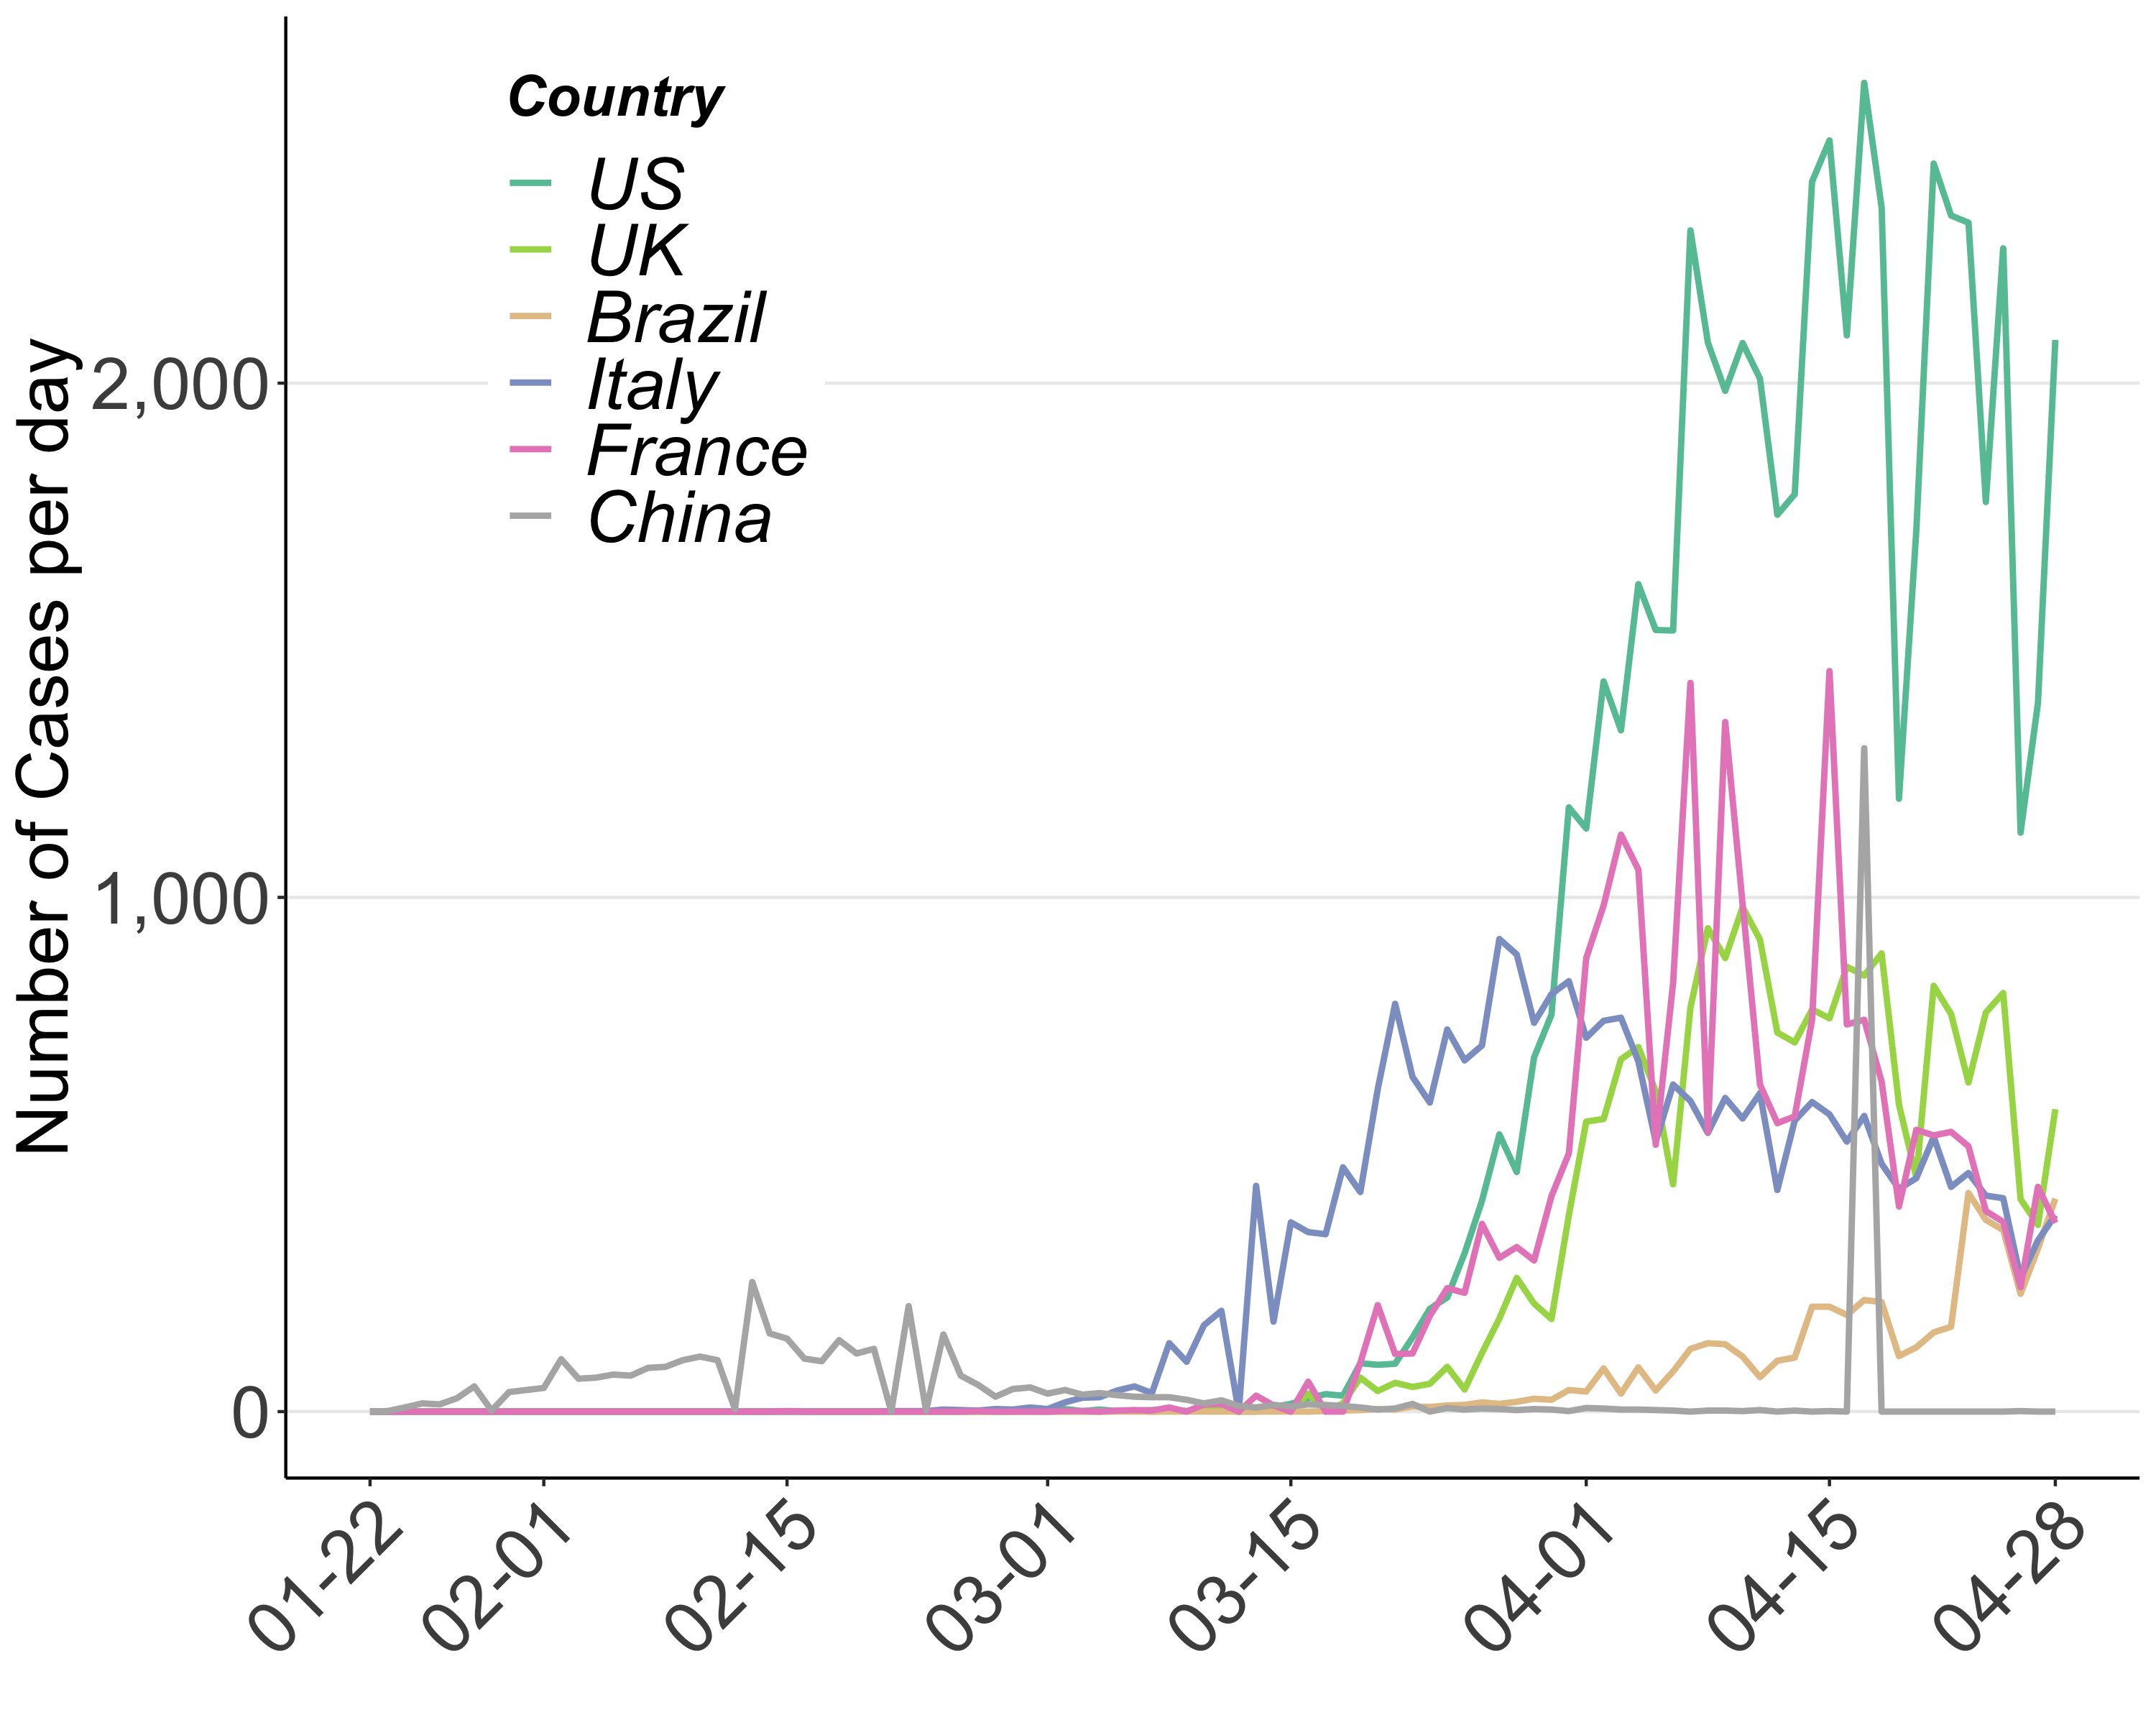
\includegraphics[]{./input/covid3.png}
\end{figure}

\vspace{-7mm}

\hypertarget{section-3}{%
\section{\texorpdfstring{\textcolor{glaucous}{\Huge 二、美国疫情}}{}}\label{section-3}}

\vspace{-5mm}

\(\bullet\)截至北京时间7月3日早8:00,
美国累计确诊病例数为2,735,554例,累计128,684死亡病例(表3和表5为霍普金斯大学官网截至北京时间7月3日早8:00所更新的数据)。

\(\quad\)\(\diamond\)共有39个州累计确诊病例超过1万例,16个州确诊病例超过5万例。

\begin{figure}[H]
\centering
\captionsetup{font={huge}}
\caption{\textcolor{grey}{美国日新增确诊前五位州趋势图}}
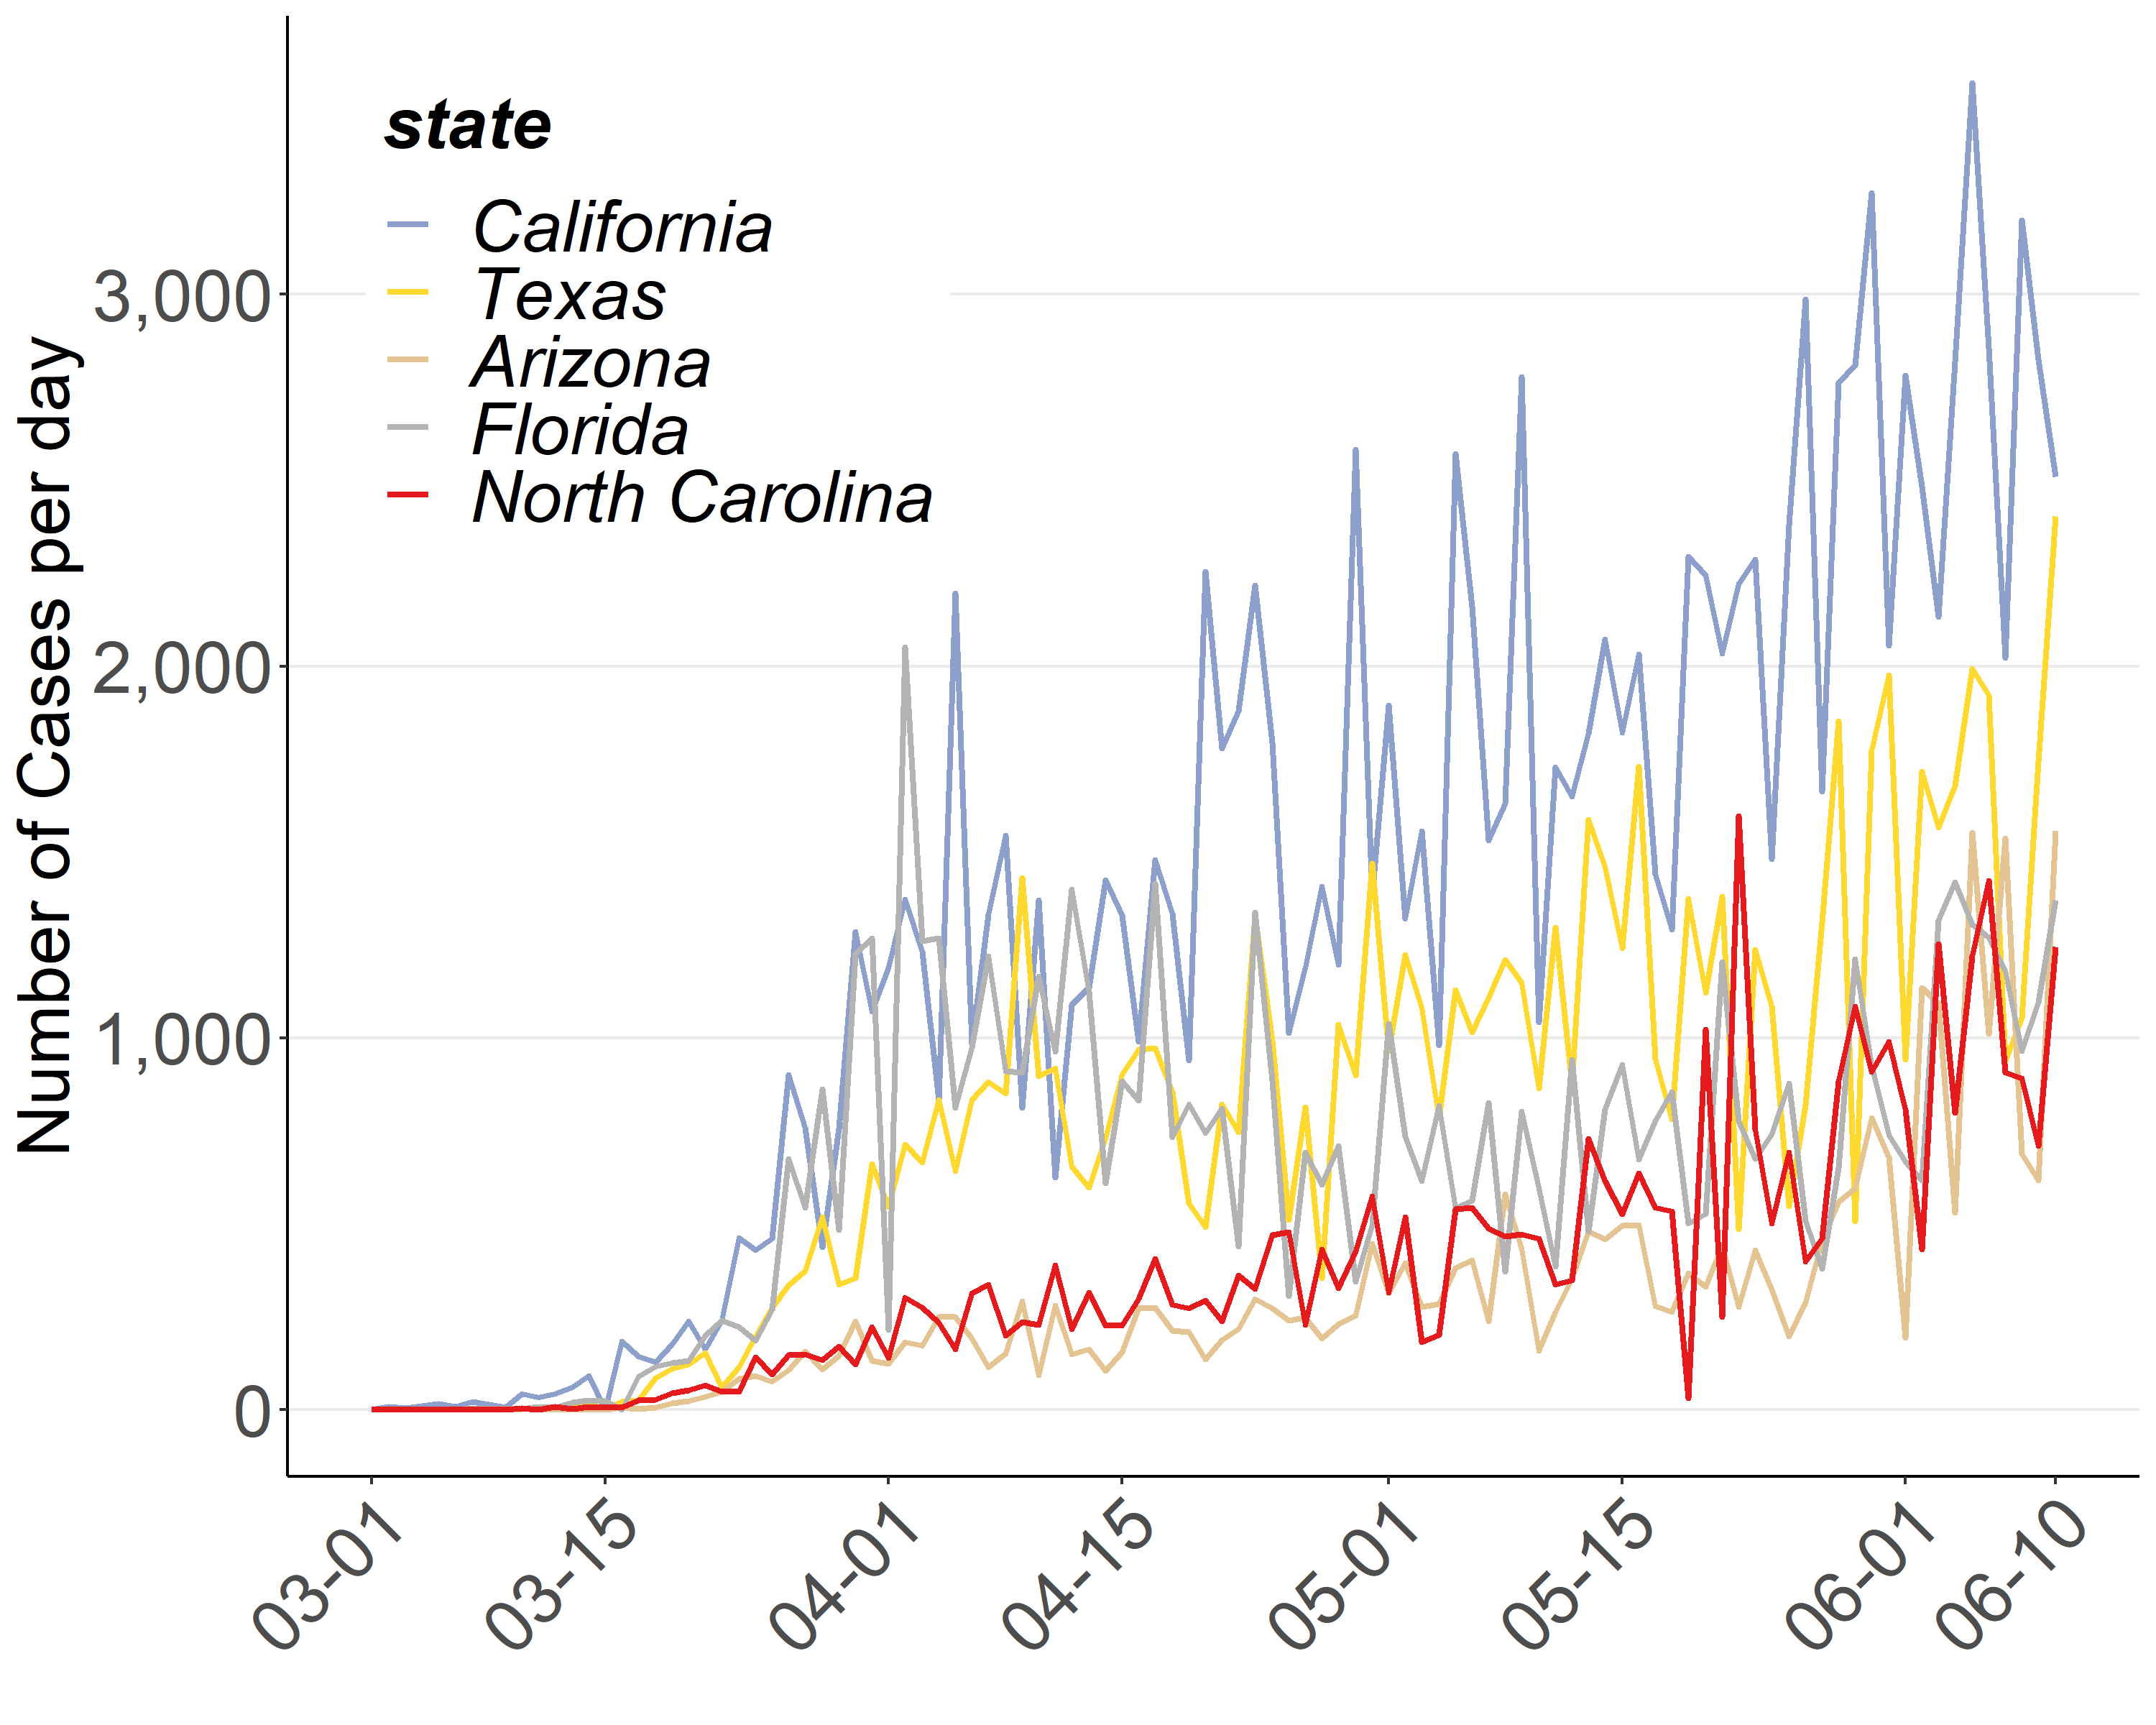
\includegraphics[]{./input/covid5.png}
\end{figure}

\begin{figure}[H]
\centering
\captionsetup{font={huge}}
\caption{\textcolor{grey}{美国日新增死亡前五位州趋势图}}
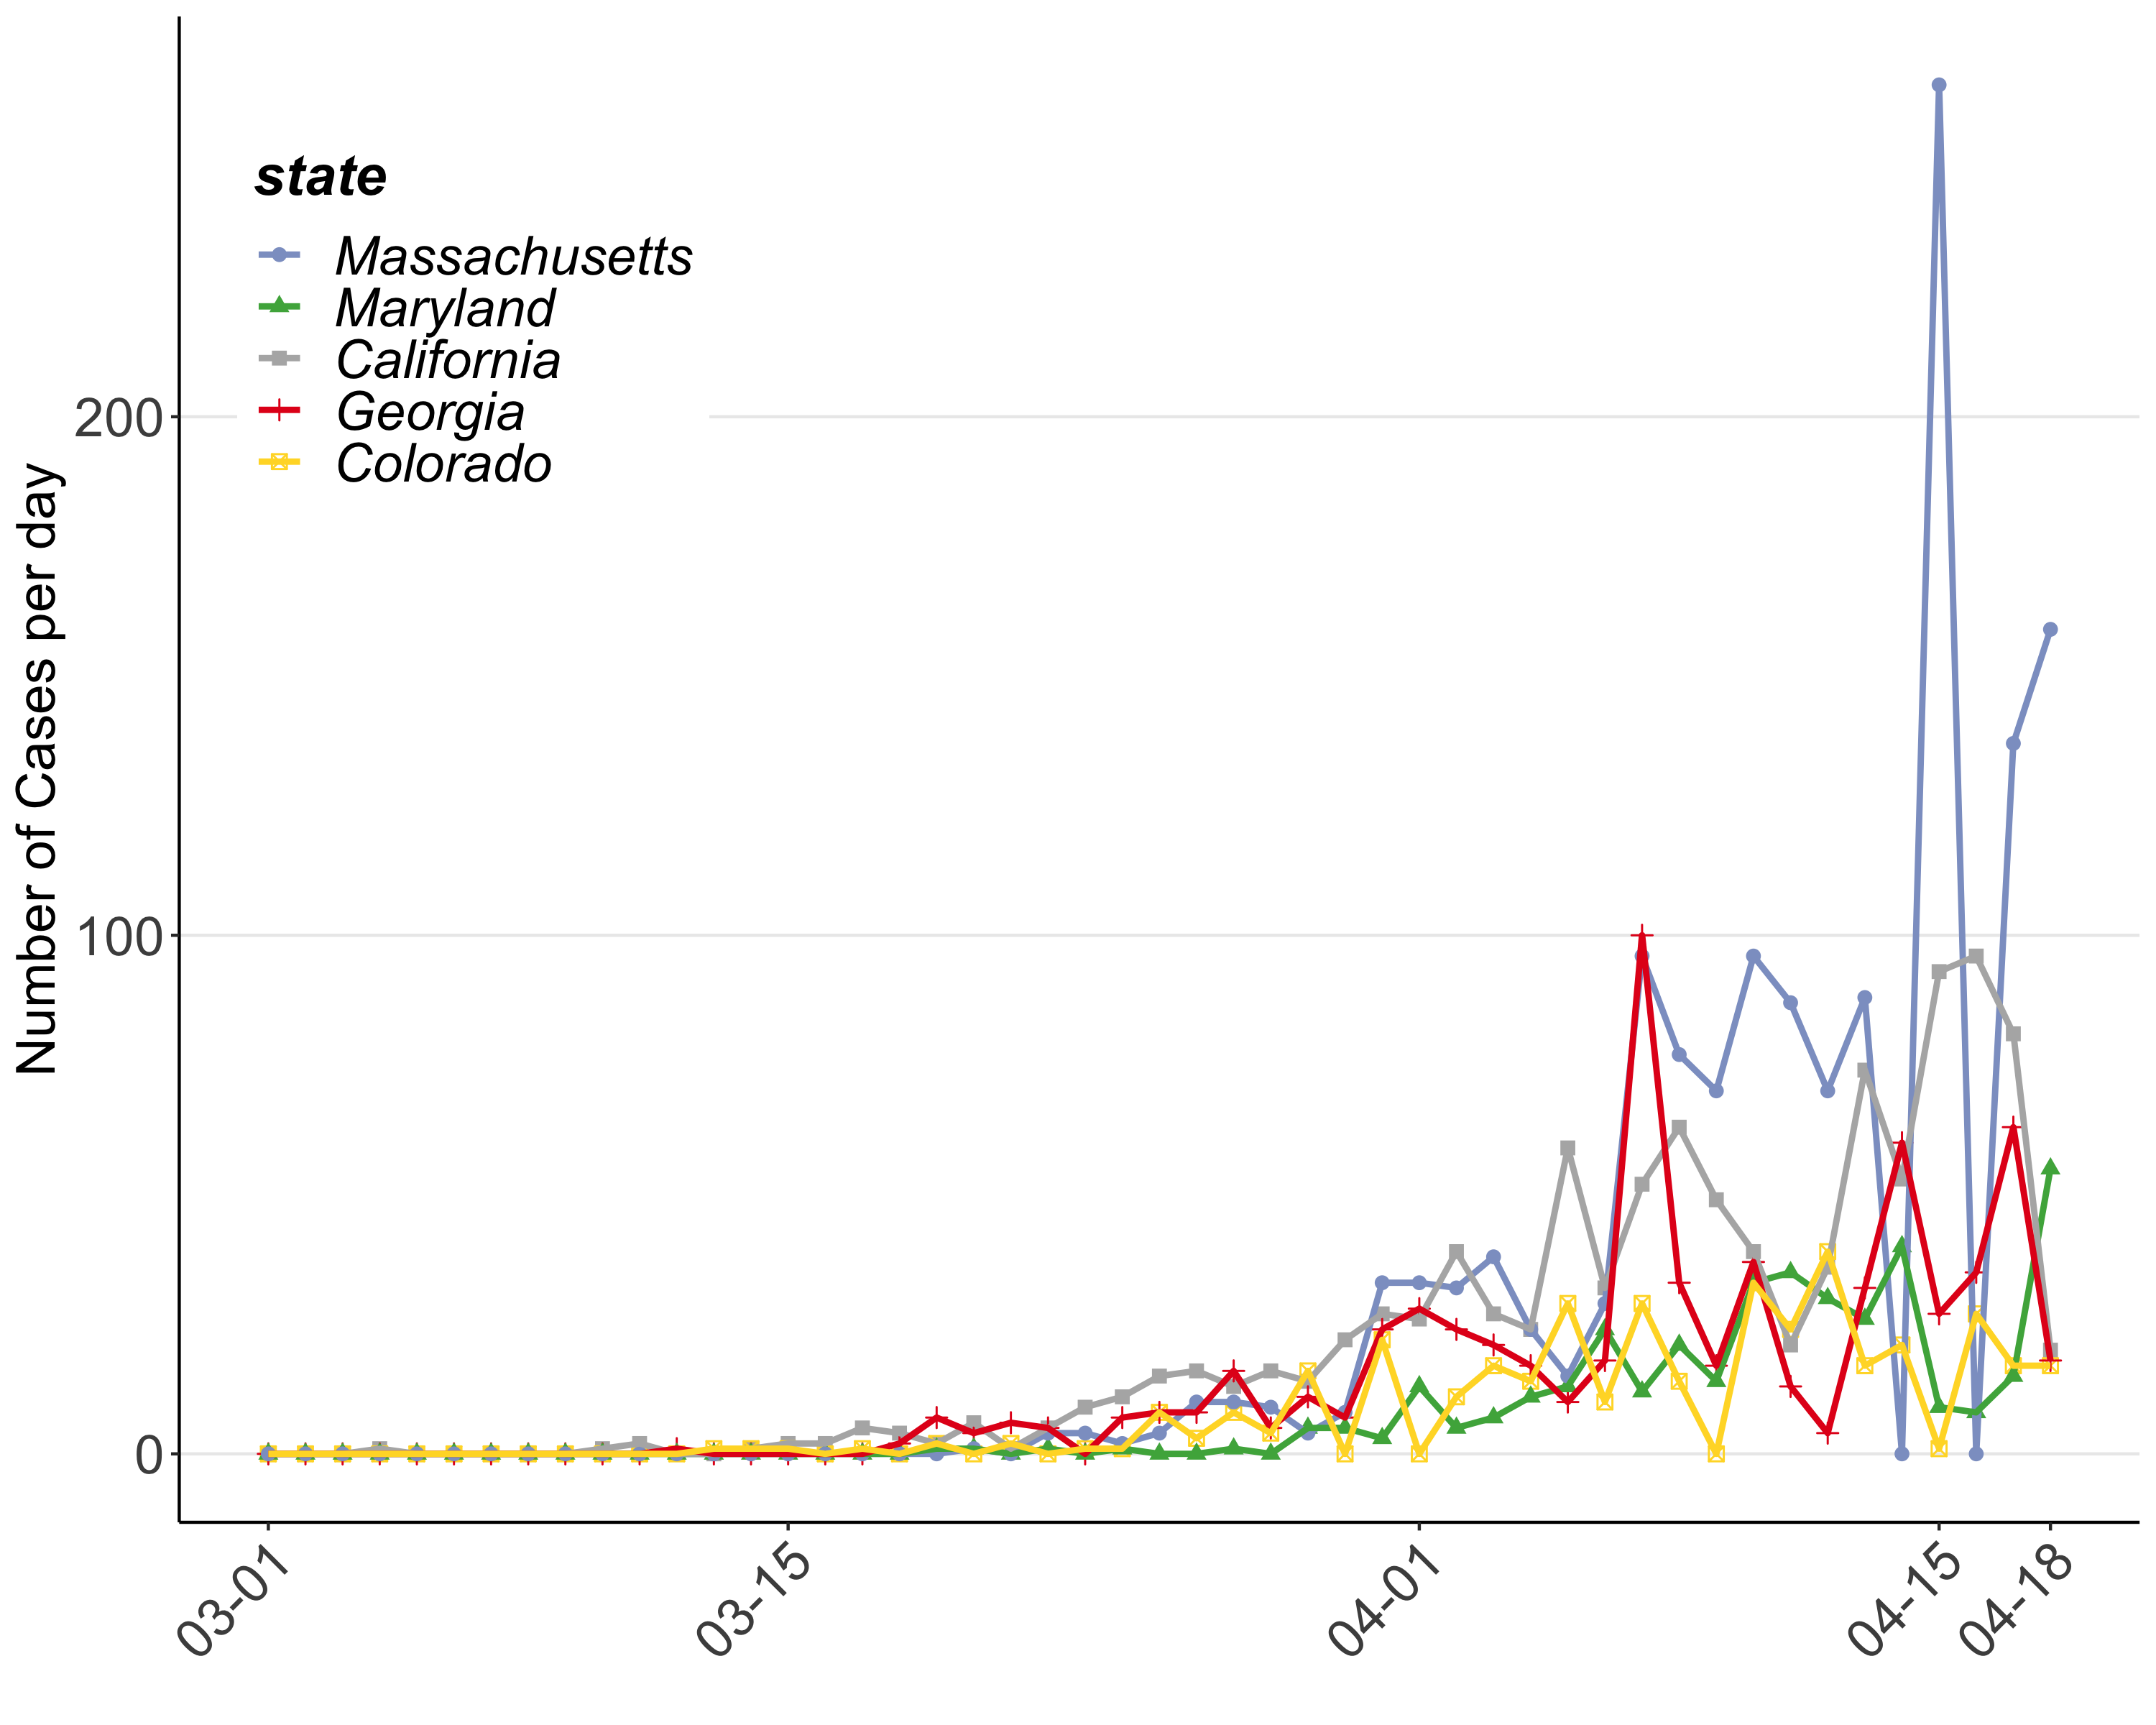
\includegraphics[]{./input/covid6.png}
\end{figure}

\begin{table}[H]
    \centering \begin{table}[H]
\centering\begingroup\fontsize{20}{22}\selectfont

\resizebox{\linewidth}{!}{
\begin{tabular}{rlrrrrrrr}
\toprule
\multicolumn{0}{c}{\textbf{ }} & \multicolumn{8}{c}{\textbf{表5 美国新增确诊前十位州}} \\
  & 国家/州名 & 累计确诊 & 粗发病率 & 累计检测 & 累计阳性率\% & 日新增检测 & 新增中阳性率\% & 检测率*\\
\midrule
\rowcolor{gray!6}   & 美国 US & 1,662,302 & 502 & 14,603,530 & 11 & 441,248 & 4 & 4,412\\
1 & 纽约州 NY & 362,764 & 1,865 & 1,739,449 & 21 & 39,623 & 3 & 8,942\\
\rowcolor{gray!6}  2 & 新泽西州 NJ & 155,092 & 1,746 & 623,797 & 25 & 19,990 & 5 & 7,023\\
3 & 伊利诺伊州 IL & 112,017 & 884 & 769,564 & 15 & 21,643 & 8 & 6,073\\
\rowcolor{gray!6}  4 & 加利福尼亚州 CA & 96,400 & 244 & 1,644,102 & 6 & 61,357 & 3 & 4,161\\
5 & 马萨诸塞州 MA & 93,271 & 1,342 & 540,561 & 17 & 8,188 & 7 & 7,778\\
\rowcolor{gray!6}  6 & 宾夕法尼亚州 PA & 71,925 & 562 & 403,114 & 18 & 7,019 & 7 & 3,149\\
7 & 得克萨斯州 TX & 56,409 & 195 & 805,654 & 7 & 42,109 & 1 & 2,779\\
\rowcolor{gray!6}  8 & 密歇根州 MI & 54,881 & 550 & 472,860 & 12 & 21,628 & 1 & 4,735\\
9 & 佛罗里达州 FL & 51,746 & 241 & 908,235 & 6 & 37,000 & 2 & 4,229\\
\rowcolor{gray!6}  10 & 马里兰州 MD & 47,152 & 780 & 249,577 & 19 & 9,215 & 9 & 4,128\\
\bottomrule
\end{tabular}}
\endgroup{}
\end{table} \end{table}\begin{table}[H]
    \centering \begin{table}[H]
\centering\begingroup\fontsize{20}{22}\selectfont

\begin{tabular}{rlrr}
\toprule
\multicolumn{0}{c}{\textbf{ }} & \multicolumn{3}{c}{\textbf{表6 美国新增死亡前十位州}} \\
  & 国家/州名 & 当日新增 & 构成比\%\\
\midrule
\rowcolor{gray!6}   & 美国 US & 23,403 & 100\\
1 & 纽约州 NY & 3,110 & 13\\
\rowcolor{gray!6}  2 & 新泽西州 NJ & 2,668 & 11\\
3 & 伊利诺伊州 IL & 2,219 & 9\\
\rowcolor{gray!6}  4 & 马萨诸塞州 MA & 1,840 & 8\\
5 & 宾夕法尼亚州 PA & 1,579 & 7\\
\rowcolor{gray!6}  6 & 加利福尼亚州 CA & 1,067 & 5\\
7 & 密歇根州 MI & 1,052 & 4\\
\rowcolor{gray!6}  8 & 得克萨斯州 TX & 901 & 4\\
9 & 弗吉尼亚州 VA & 801 & 3\\
\rowcolor{gray!6}  10 & 佛罗里达州 FL & 710 & 3\\
\bottomrule
\end{tabular}
\endgroup{}
\end{table} \begin{tablenotes}
        \fontsize{15}{15}
        \selectfont
        \item 
      \end{tablenotes}
\end{table}

\(\bullet\)美国昨日新增确诊47,751例(图4和表5),新增死亡572例(图5和表6)。单日新增排名前十位的州昨日新增确诊均超过1,000例,共39个州累计确诊超过10,000例。

\(\quad\)\(\diamond\)佛罗里达州单日新增确诊病例再创新高,接近1万(10,109)例。

\(\quad\)\(\diamond\)得克萨斯州疫情依旧不容乐观,近半个月单日新增确诊均超过4,000例。

\(\quad\)\(\diamond\)乔治亚州近来疫情进展迅速,昨日新增确诊病例为3,340例。

\vspace{5mm}

\begin{center}

\includegraphics[height=2cm]{./input/title3.png} 
\end{center}

\vspace{-5mm}

\hypertarget{section-4}{%
\section{\texorpdfstring{\textcolor{glaucous}{\Huge 明星疫苗介绍}}{}}\label{section-4}}

\vspace{-3mm}

每年4月最后一周(4月24---30日)是``世界免疫周'',其目的是促进接种疫苗以保护各年龄人群免患疾病。在新冠疫情在全球肆虐的背景下,疫苗被寄予了彻底终结疫情的厚望。3月,中国和美国几乎同时有疫苗研究宣布进入临床阶段,并且有一些中美合作共同推进的项目。现在全球正在进行的新冠疫苗研究超过100项。

下面我们来看在全球率先进入临床试验阶段的几款不同原理的新冠病毒疫苗:\(\\\)

\centerline{mRNA-1273 $^1$}

\(\\\)
全球第一个获批进入临床试验的候选疫苗为美国Moderna公司的mRNA疫苗。mRNA疫苗是指直接给人体注射病毒的编码核酸,再由人体的细胞自己合成病毒蛋白并产生免疫应答。1月13日,美国国立卫生院(NIH)和Moderna就完成该新冠病毒疫苗序列的设计,起名为
mRNA-1273。由CEPI(Coalition for Epidemic Preparedness Innovations,
防疫创新联盟)出资后Moderna启动临床生产,2月7日第一批临床生产的疫苗完成。3月4日,美国食品药品监管局(FDA)批准了mRNA-1273进入临床试验,3月16日,第一位志愿者接受了第一剂疫苗的接种。目前尚在临床I期实验阶段,并于本周开始对45名志愿者注射第二针疫苗。

\(\\\)

\centerline{Ad5-nCoV $^2$}

中国第一个获批进入临床试验的候选疫苗为重组腺病毒载体疫苗Ad5-nCoV。腺病毒疫苗的原理是把新冠病毒表面的蛋白整合到没有致病力的腺病毒的表面,以免疫刺激人体产生针对新冠病毒的抗体。Ad5-nCoV是由军事科学院军事医学研究院的陈薇院士团队与国内康希诺公司联合开发,
3月16日获国家药品监督局批准展开I期临床试验,并于4月9日公布I期临床试验108名志愿者的初步安全数据,并宣布进入临床II期。

\(\\\)

\centerline{INO-4800 $^3$}

全球第三款进入临床试验阶段的新冠疫苗,也是第一个候选的DNA疫苗,是来自Inovio
Pharmaceuticals公司的INO-4800。DNA疫苗原理与mRNA疫苗相同,目前已用于艾滋病毒、流感病毒、疟疾等多种疫苗的开发。Inovio在获得病毒基因序列后在三个小时内就完成了疫苗设计。1月30日,Inovio公司宣布与中国国内企业艾棣维欣达成合作协议,共同推进INO-4800在中国的研发工作。4月7日,美国食品药品监管局(FDA)接受该公司为新冠病毒候选DNA疫苗递交的新药临床试验(IND)申请灭活病毒疫苗。Inovio于4月29日宣布其在美国招收的40名志愿者已经完成第一轮疫苗注射。

\(\\\)

\centerline{新冠病毒灭活疫苗 $^4$}

全球第一个灭活病毒疫苗由国药集团下武汉生物制品研究所有限责任公司与中科院武汉病毒所研发。灭毒活疫苗的原理是杀死病毒以使其失去致病力,但保留病毒表面的蛋白质,使其注射入体内后依然可以刺激免疫反应。2月1日,该项目获得科技部国家重点研发计划``公共安全风险防控与应急技术装备''重点专项``2019-nCoV灭活疫苗''的紧急立项。在4月12日获得了国家药品监督管理局临床试验许可,已开展随机、双盲、安慰剂平行对照I/II期临床试验。

\vspace{5mm}

\Large \(\\\)参考文献:

1 Safety and Immunogenicity Study of 2019-nCoV Vaccine (mRNA-1273) for
Prophylaxis SARS CoV-2 Infection
(COVID-19).https://www.clinicaltrials.gov/ct2/show/NCT04283461 2.Phase I
Clinical Trial of a COVID-19 Vaccine in 18-60 Healthy Adults
(CTCOVID-19). \url{https://clinicaltrials.gov/ct2/show/NCT04313127}
3.Safety, Tolerability and Immunogenicity of INO-4800 for COVID-19 in
Healthy Volunteers.
\url{https://clinicaltrials.gov/ct2/show/NCT04336410} 4.斥资10亿元
国药集团新冠疫苗研发领跑全球.
\url{http://www.xinhuanet.com/2020-04/27/c_1125909948.htm}

\vspace{5mm}

\centering
\fontsize{12}{12}
\selectfont
\begin{tabular}{ll}


主编:马晶  &  副主编:仁晖,史珂玮 \\
责任编辑: 霍舒同  \\
新闻组: 闫怡璇 &  数据分析:韩佩瑾 \\
热点话题:朱诗韵 & 微信排版:韩佩瑾 \\
\multicolumn{2}{l}{可视化组:张立达\, 孙昊\, 唐星鸿\, 齐维为\, 刘逸洋\, 张祺珉\, 周梓淇}

\end{tabular}

\end{document}
